% Copyright (C) 2021 Diogo Rodrigues, Rafael Ribeiro, Bernardo Ferreira
% Distributed under the terms of the GNU General Public License, version 3

\documentclass{beamer}
% Encodings (to render letters with diacritics and special characters)
\usepackage[utf8]{inputenc}
% Language
\usepackage[english]{babel}
\usepackage{verbatim}

\usepackage{csvsimple}

\usetheme{Madrid}
\usecolortheme{default}

\pdfstringdefDisableCommands{
  \def\\{}
  \def\texttt#1{<#1>}
}

\newcommand{\email}[1]{
{\footnotesize \texttt{\href{mailto:#1}{#1}} }
}

\usepackage{caption}
\DeclareCaptionFont{black}{\color{black}}
\DeclareCaptionFormat{listing}{{\tiny \textbf{#1}#2#3}}
\captionsetup[lstlisting]{format=listing,labelfont=black,textfont=black}

\usepackage{listings}
\lstset{
    frame=tb, % draw frame at top and bottom of the code
    basewidth  = {0.5em,0.5em},
    numbers=left, % display line numbers on the left
    showstringspaces=false, % don't mark spaces in strings  
    commentstyle=\color{green}, % comment color
    keywordstyle=\color{blue}, % keyword color
    stringstyle=\color{red}, % string color
	aboveskip=-0.2em,
    belowskip=-0.2em,
    basicstyle=\tiny
}
\lstset{literate=
  {á}{{\'a}}1 {é}{{\'e}}1 {í}{{\'i}}1 {ó}{{\'o}}1 {ú}{{\'u}}1
  {Á}{{\'A}}1 {É}{{\'E}}1 {Í}{{\'I}}1 {Ó}{{\'O}}1 {Ú}{{\'U}}1
  {à}{{\`a}}1 {è}{{\`e}}1 {ì}{{\`i}}1 {ò}{{\`o}}1 {ù}{{\`u}}1
  {À}{{\`A}}1 {È}{{\'E}}1 {Ì}{{\`I}}1 {Ò}{{\`O}}1 {Ù}{{\`U}}1
  {ä}{{\"a}}1 {ë}{{\"e}}1 {ï}{{\"i}}1 {ö}{{\"o}}1 {ü}{{\"u}}1
  {Ä}{{\"A}}1 {Ë}{{\"E}}1 {Ï}{{\"I}}1 {Ö}{{\"O}}1 {Ü}{{\"U}}1
  {â}{{\^a}}1 {ê}{{\^e}}1 {î}{{\^i}}1 {ô}{{\^o}}1 {û}{{\^u}}1
  {Â}{{\^A}}1 {Ê}{{\^E}}1 {Î}{{\^I}}1 {Ô}{{\^O}}1 {Û}{{\^U}}1
  {Ã}{{\~A}}1 {ã}{{\~a}}1 {Õ}{{\~O}}1 {õ}{{\~o}}1
  {œ}{{\oe}}1 {Œ}{{\OE}}1 {æ}{{\ae}}1 {Æ}{{\AE}}1 {ß}{{\ss}}1
  {ű}{{\H{u}}}1 {Ű}{{\H{U}}}1 {ő}{{\H{o}}}1 {Ő}{{\H{O}}}1
  {ç}{{\c c}}1 {Ç}{{\c C}}1 {ø}{{\o}}1 {å}{{\r a}}1 {Å}{{\r A}}1
  {€}{{\euro}}1 {£}{{\pounds}}1 {«}{{\guillemotleft}}1
  {»}{{\guillemotright}}1 {ñ}{{\~n}}1 {Ñ}{{\~N}}1 {¿}{{?`}}1
}

\usepackage{dirtree}

\usepackage[style=british]{csquotes}

\usepackage{tabularx}
\usepackage{multirow}

\usepackage{multicol}

\usepackage{graphicx}
	\graphicspath{{./images/}{../documentacao/}}

\usepackage[binary-units=true]{siunitx}

\usepackage{pgfplots, pgfplotstable}
\newcommand{\errorband}[5][]{ % x column, y column, error column, optional argument for setting style of the area plot
    \pgfplotstableread[col sep=comma]{#2}{\datatable}
    % Lower bound
    \addplot [draw=none, stack plots=y, forget plot] table [
      x={#3},
      y={#4},
    ] {\datatable};

    \addplot [draw=none, fill=gray!40, stack plots=y, area legend, #1] table [
      x={#3},
      y expr=\thisrow{#5}-\thisrow{#4}+1e-4,
    ] {\datatable} \closedcycle;

    % Reset stack
    \addplot [forget plot, stack plots=y,draw=none] table [
      x={#3},
      y expr=-\thisrow{#5}-1e-4,
    ] {\datatable};
}

\pgfplotsset{
  compat=1.16,
  title style={font=\bfseries},
  label style={font=\small},
  tick label style={font=\footnotesize},
  legend style={
    font=\scriptsize,
    row sep=-1pt,
  },
  legend cell align={left},
}
 
%Information to be included in the title page:
\AtBeginDocument{
\title[Ball Sort Puzzle (final delivery)]{Ball Sort Puzzle}
\subtitle[]{Final delivery}
\author[Group 48]{
\begin{tabular}{r l}
	\email{up201806581@fe.up.pt} & Bernardo António Magalhães Ferreira \\
	\email{up201806429@fe.up.pt} & Diogo Miguel Ferreira Rodrigues     \\
	\email{up201806330@fe.up.pt} & Rafael Soares Ribeiro
\end{tabular}
}
\institute[FEUP/IART]{Faculdade de Engenharia da Universidade do Porto \\ Artificial Intelligence (IART) -- Group 48}
\date[03/04/2021]{3rd of April, 2021}
}

\begin{document}
\frame{\titlepage}

\begin{frame}
\frametitle{1. Work specification}
\framesubtitle{1.1. Problem description}

Solve solitaire game \href{https://play.google.com/store/apps/details?id=com.spicags.ballsort&hl=pt_PT&gl=US}{\textit{Ball Sort Puzzle}} by \href{https://play.google.com/store/apps/developer?id=Spica+Game+Studio}{Spica Game Studio} heuristic search methods.

Starting with a set of differently coloured balls distributed at random in different tubes, sort them so each tube has balls of a single color.

\vspace{0.5em}

\begin{minipage}{0.42\textwidth}
  \begin{itemize}
    \itemsep0em
    \item There are more tubes than colors;
    \item There are as many balls of a color as can fit in a tube;
    \item Cannot place more balls in a tube than it can hold;
    \item Can only move a ball on top of same-color ball (or tube is empty).
  \end{itemize}
\end{minipage}%
\begin{minipage}{0.58\textwidth}
  \centering
  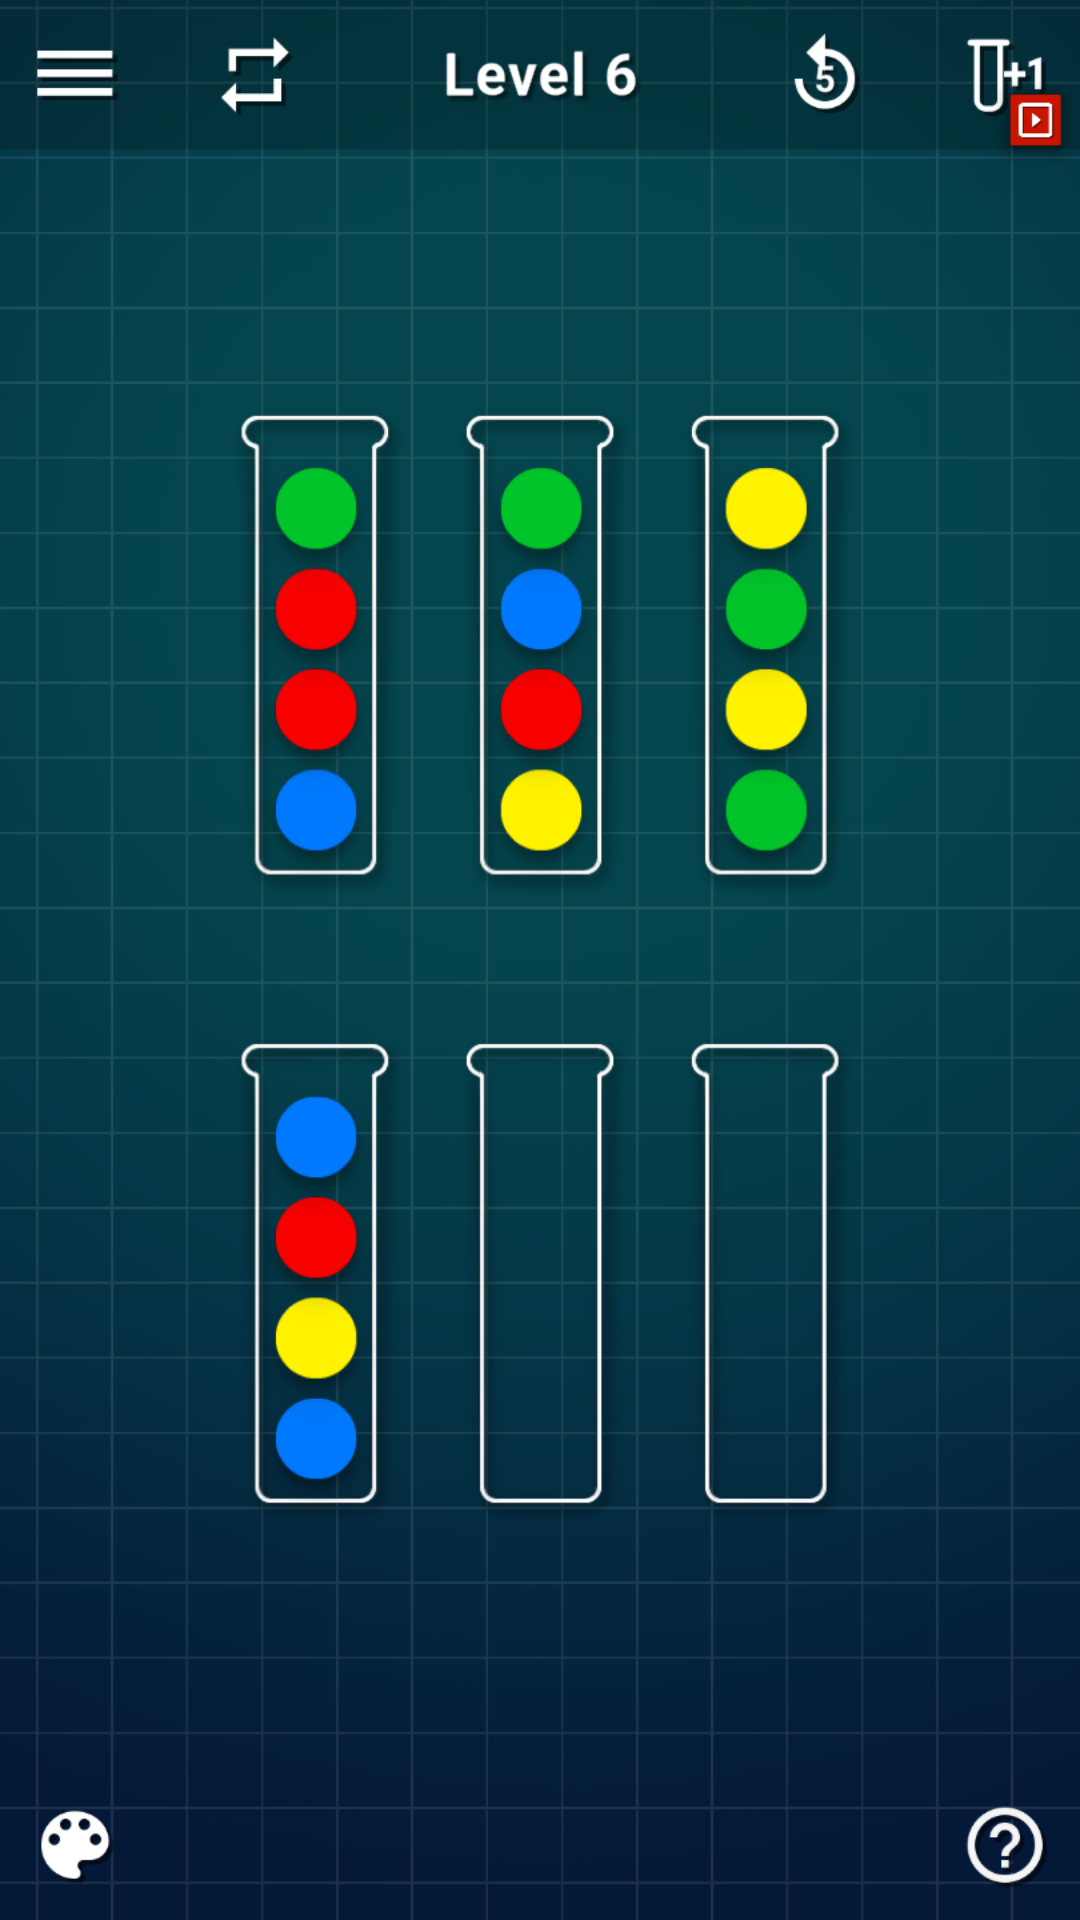
\includegraphics[width=29mm]{img/lvl6-begin.png}
  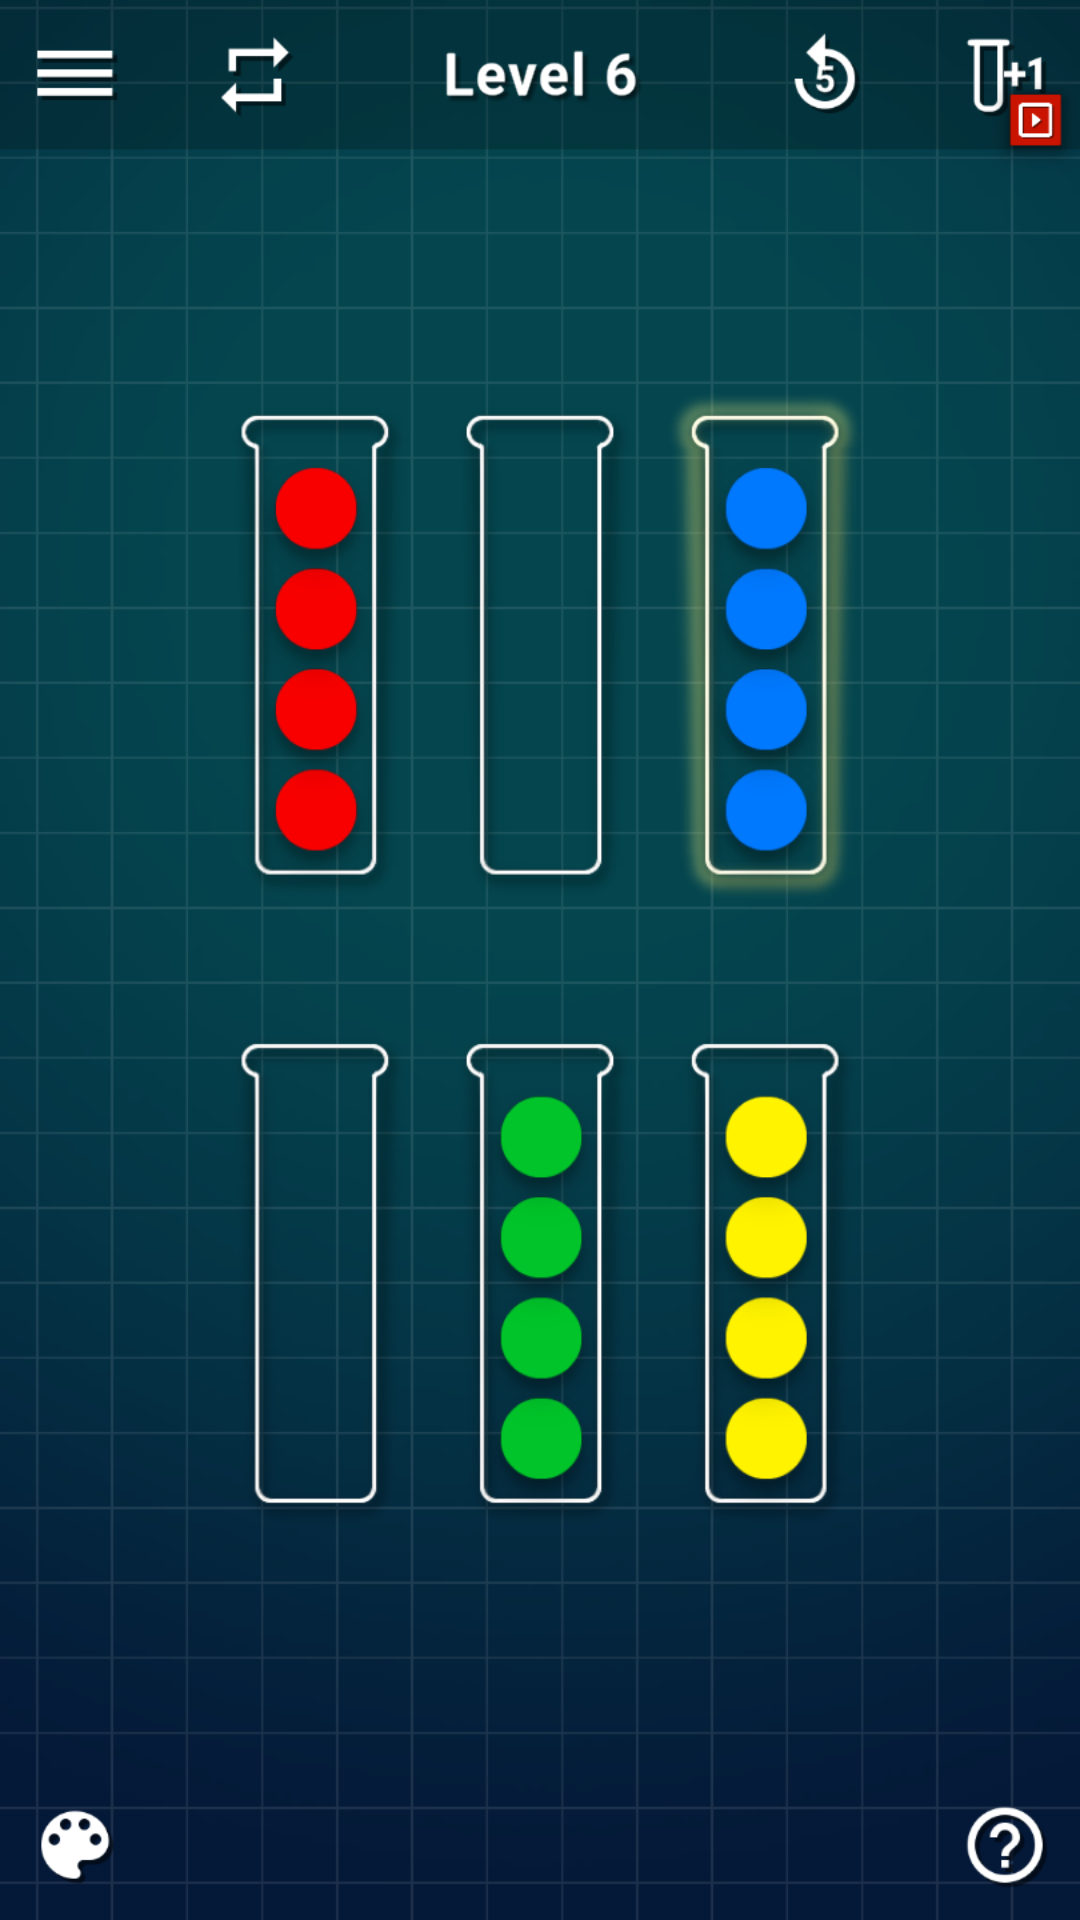
\includegraphics[width=29mm]{img/lvl6-end.png}
\end{minipage}

\end{frame}

\begin{frame}
\frametitle{1. Work specification}
\framesubtitle{1.2. Solution description}

\begin{enumerate}
  \itemsep0em
  \item Implement the game and a human-friendly interface.
  \item Implement search algorithms to solve the game, and compare performances. These algorithms are used to search for a path to a solution in a tree of game states.

  \begin{itemize}
    \itemsep0em
    \item We can use uninformed search algorithms (BFS, DFS, iterative deepening, uniform cost) and informed search algorithms (greedy search, A* algorithm).
  \end{itemize}
\end{enumerate}

\end{frame}

\begin{frame}
\frametitle{2. Related works}

A few common problems related to stacks, mostly applied to cargo containers.

Assume there is a set of cargo containers in a yard with a certain number of slots, and that containers are stacked to save space.

\vspace{0.5em}

\begin{tabular}{@{}p{46mm} p{70mm}@{}}
  \textbf{Container Pre-Marshalling Problem (CPMP)} & \textbf{Block Relocation Problem (BRP)} \\
  Some containers have more priority than others (e.g., are meant to be shipped first than others), so each stack must be sorted in non-decreasing order of priority from the bottom up with the least number of moves. &
  Containers will be extracted in a specific order (say that the $N$ containers are numbered from $1$ to $N$; container 1 is extracted first, then 2, ..., and finally container $N$). The goal is to extract all containers in that order with the least amount of moves (i.e., if you need to remove container 3 to extract container 1, you'd prefer to put 3 on top of 4 than on top of 2, otherwise you'd have to again relocate 3 to reach 2).
\end{tabular}

\end{frame}

\begin{frame}
\begin{itemize}
\item In both problems, search methods such as A* (with carefully considered heuristics) and branch-and-bound are regularly applied and yield good results, although optimal methods are clearly only reasonable in small scenarios, or to evaluate quality of sub-optimal, faster heuristic search methods.

\item \cite{bortfeldt2012} provided a lower bound for the number of moves (very important to use as admissible heuristic for A*), and applied a tree search procedure to CPMP. \cite{tierney2017} further applied branching/symmetry breaking rules and iterative deepening A* to increase the size of problems that can be solved optimally.

\item \cite{tricoire2018} proposed heuristics/metaheuristics for large BRP instances, and compared those approaches to branch-and-bound algorithms.
\end{itemize}

This research is significant for our problem; even though the problems are quite different in nature, they share some traits with our problem, and can contribute with ideas for our own heuristics.

\end{frame}

\begin{frame}[fragile=singleslide]
\frametitle{3. Formulation}
\framesubtitle{3.1. Game definition}

\textbf{Game state} | Vector $S = \langle t_1, t_2, ..., t_N \rangle$ of $N$ tubes with maximum capacity $H$, where tube $i$ is a stack $t_i = \langle t_i(1), t_i(2), ..., t_i(h_i) \rangle$ with $h_i$ balls ($0 \leq h_i \leq H$), where $t_i(1)$ is the color of the ball at the bottom, and $t_i(h_i)$ the color at the top. There are $C$ colors ($C < N$) numbered sequentially, thus $\forall i, j,~1 \leq t_i(j) \leq C$.

\textbf{Initial state} | The balls are randomly distributed over the tubes.

\textbf{Objective test} | For each tube, the tube is empty or all balls on that tube have the same color.

\textbf{Operators} | The only operator is a move:
\begin{itemize}
  \item Given state $S$, choose origin \& destination tubes $1 \leq i, j \leq N$ ($i \neq j$).
  \item Pre-conditions: $h_i \geq 1$, $h_j < H$ and either $h_j = 0$ or $t_i(h_i)=t_j(h_j)$.
  \item Cost: $1$ (one).
  \item Post-conditions: $S'$ is built from $S$, except $t_i$ is a ball shorter (say it had color $c$), and $t_j$ has one more ball at the top with color $c$.
\end{itemize}

\end{frame}

\begin{frame}
  \frametitle{3. Formulation}
  \framesubtitle{3.2. Heuristics}
  This heuristic will describe an estimate of the distance to a solution in \# of moves:
  \begin{itemize}
    \item For each tube, add the number of balls in that tube that have a different color than the last ball in the tube.
    \item Number of balls in the $N-C$ tubes with least balls.
    \item If there are two tubes with same color at the bottom, we will need at least the additional number of moves required to move pieces from one side to another
  \end{itemize}

  Other ideas:
  \begin{itemize}
    \item Double that heuristic, to reach a solution faster although A* becomes sub-optimal.
  \end{itemize}
\end{frame}

\begin{frame}
\frametitle{4. Implementation}

\small

\vspace{-0.5em}

\setlength{\multicolsep}{6.0pt plus 2.0pt minus 1.5pt}% 50% of original values
\begin{multicols}{2}

  \textbf{Language} | C++

  \textbf{Environment} | Compiled with CMake, terminal interface

  \textbf{Data structures} | \texttt{color\_t} is a \texttt{typedef} for an \texttt{int}, game state represented as \texttt{vector<deque<color\_t>>}

  \textbf{File structure} | No input from files; project is being developed using an MVC model with small but useful functions

\end{multicols}

\textbf{Summary:} implemented UI, integrated search methods in UI, allows hints; implemented CLI to run batches to evaluate performance.

\begin{center}
  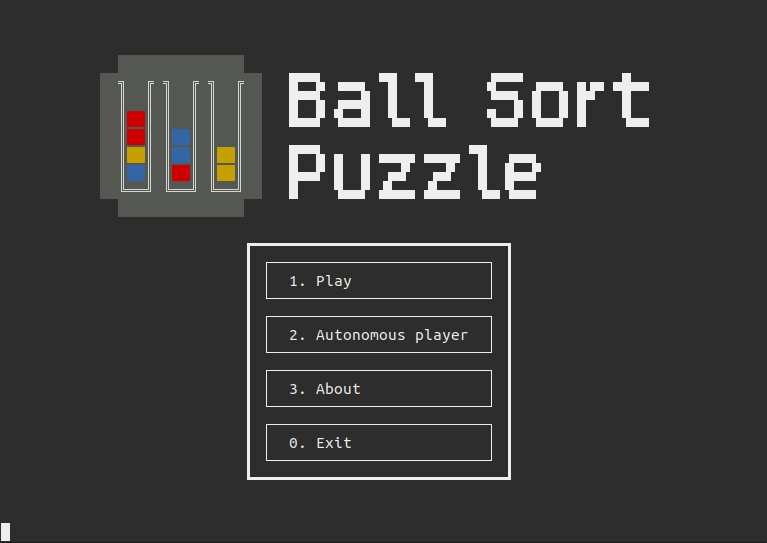
\includegraphics[height=40mm]{img/main-menu.png}
  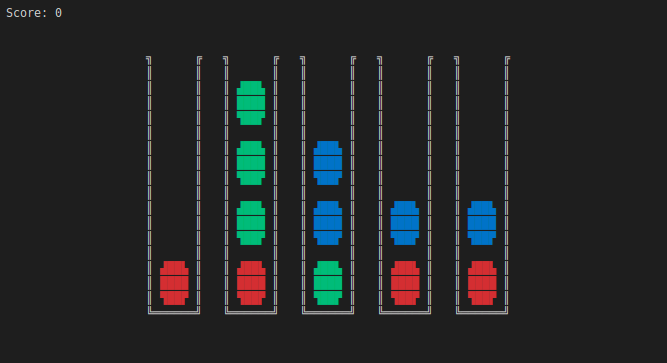
\includegraphics[height=40mm]{img/game-interface.png}
\end{center}

\end{frame}

\begin{frame}
\frametitle{6. Implemented algorithms}
\framesubtitle{6.1. Uninformed search methods}

\begin{itemize}
  \item \textbf{Depth First Search (DFS)} | Starting in a given node, expands its children in a random order until if finds that branch does not have a solution, and backtracks until it finds another branch to explore. 
  
  \item \textbf{Breadth First Search (BFS)} |  Expand the non-expanded node closest to the origin. Keeps queue with frontier nodes (visited but not expanded), expands the node at the front of the queue and pushes new frontier nodes to the back.
  
  \item \textbf{Iterative Deepening Search (IDS)} | DFS with limited depth $d$; starts at $0$ and is incremented until a solution is found. Slower than BFS, but takes less memory when branching factor is large.
  
  \item \textcolor{gray}{\textbf{Uniform Cost Search (UCS)} | Variation of Dijkstra's algorithm, assumes an infinite number of states, so only adds nodes to queue as they are visited.
  UCS is equivalent to BFS if all transitions have the same cost \cite{javatpoint-uninformed}.
  Since we only have one operator with cost 1, we did not implement this algorithm.}
\end{itemize}
\end{frame}

\begin{frame}
  \frametitle{5. Approach}
  
  In our case, our evaluation functions are heuristics, and when an algorithm requires an heuristic we can also provide it with an evaluation function, so the terms are interchangeable.

  ~

  We implemented two heuristics:
  \begin{itemize}
    \item \textbf{Admissible heuristic} | TODO
    \item \textbf{Finite horizon heuristic} | Instead of making some math from the current state, finds all nodes at a certain depth, evaluates all those nodes against a base heuristic, and then pick the best value, adds the depth and returns that.
    It didn't work out that well, as time performance was worst by a factor of about 100 compared to a regular, 1-step heuristic, so we dropped it from performance analysis.
  \end{itemize}
  \end{frame}

\begin{frame}
\frametitle{6. Implemented algorithms}
\framesubtitle{6.2. Informed search methods}

\begin{itemize}  
  \item \textbf{Depth First Search Greedy (DFS-greedy)} | DFS, but uses an heuristic to rank nodes adjacent to current node, and expands them in increasing order of the heuristic score.
  \item \textbf{Greedy Search (Greedy)} | Best-first search, similar to BFS but the frontier is a priority queue, and priority is given by an heuristic instead of being the distance from the origin to that node.
  \item \textbf{A* Algorithm (A*)} | Similar to Greedy Search, but heuristic is considered an estimate of \# of moves to reach any goal state; priority of a node $u$ is the estimated total length of a solution passing through $u$ (i.e., the minimum distance from origin to $u$ plus the estimated distance from $u$ to any goal state).
\end{itemize}
\end{frame}

\begin{frame}
  \frametitle{7. Results}
  \framesubtitle{7.1. Preliminary results}
  \small

  Seed is 0, time measurements averaged over 10 executions.

  \textbf{Optimality} | Quotient of optimal solution by obtained solution. $1$ means optimal, $<1$ means sub-optimal.

  (Dashes represent computations longer than reasonable time limits)

  ~

  \begin{minipage}[c]{0.77\textwidth}
    \begin{figure}
      \centering
      \scriptsize
      \sisetup{round-mode=places
        ,round-precision=3
        ,scientific-notation=fixed
        ,fixed-exponent=0
      }
      \setlength{\tabcolsep}{0.45em}
      \begin{tabular}{r | r | r || r || l | l | l | p{3.0em} | l | l}
        & & & &
        \multicolumn{6}{c}{\textbf{Optimality}} \\ \cline{5-10}
        \rotatebox[origin=c]{90}{\textbf{\# of tubes}}
        & \rotatebox[origin=c]{90}{\textbf{Tube height}}
        & \rotatebox[origin=c]{90}{\textbf{\# of colors}}
        & \begin{minipage}{3.5em}\textbf{Optimal solution}\end{minipage}
        & \textbf{DFS}
        & \textbf{BFS}
        & \textbf{IDS}
        & \textbf{DFS-greedy}
        & \textbf{Greedy}
        & \textbf{A*}
        \csvreader[head to column names]{../../analysis/discard-dfs/discard-dfs-math.csv}{}
        {\\\hline
          \nTubes
          & \tubeH
          & \nColors
          & $\num{\astaradmissiblenMoves}$
          & $\num{\dfsnMoves}$
          & $\num{\bfsnMoves}$
          & \ifthenelse{\equal{\iterativedeepeningnMoves}{\string -}}{
            -
          }{
            $\num{\iterativedeepeningnMoves}$
          }
          & $\num{\dfsgreedyadmissiblenMoves}$
          & $\num{\greedyadmissiblenMoves}$
          & $\num{1}$
        }
      \end{tabular}
      \caption{Optimality of several methods.}
    \end{figure}
  \end{minipage}
  \begin{minipage}[c]{0.22\textwidth}
    \textbf{Optimal:}
    \begin{itemize}
      \itemsep0em
      \item BFS
      \item IDS
      \item A*
    \end{itemize}
    \textbf{Near-optimal:}
    \begin{itemize}
      \itemsep0em
      \item DFS-greedy
      \item Greedy
    \end{itemize}
    \textbf{Awful:}
    \begin{itemize}
      \itemsep0em
      \item DFS
    \end{itemize}
  \end{minipage}

\end{frame}

\begin{frame}
  Since BFS is the slowest optimal method, we used it to compare performance.
  \begin{figure}
    \centering
    \scriptsize
    \sisetup{round-mode=places
      ,round-precision=3
      ,round-minimum  = 0.001
      ,scientific-notation=fixed
      ,fixed-exponent=0
    }  
    \setlength{\tabcolsep}{0.45em}
    \begin{tabular}{r | r | r || r || r | r | r | r | r}
      &
      &
      &
      &
      \multicolumn{5}{c}{\textbf{Execution time} (as multiple of BFS execution time)} \\ \cline{5-9}

      \rotatebox[origin=c]{90}{\textbf{\# of tubes}}
      & \rotatebox[origin=c]{90}{\textbf{Tube height}}
      & \rotatebox[origin=c]{90}{\textbf{\# of colors}}
      & \begin{minipage}{5.0em}\textbf{BFS exec. time ($\si{\milli\second}$)}\end{minipage}
      & \textbf{DFS}
      & \textbf{IDS}
      & \textbf{DFS-greedy}
      & \textbf{Greedy}
      & \textbf{A*}
      \csvreader[head to column names]{../../analysis/discard-dfs/discard-dfs-math.csv}{}
      {\\\hline
        \nTubes
        & \tubeH
        & \nColors
        & $\num[round-precision=2]{\bfstns}$
        & $\num{\dfstns}$
        & \ifthenelse{\equal{\iterativedeepeningtns}{\string -}}{
          -
        }{
          $\num{\iterativedeepeningtns}$
        }
        & $\num{\dfsgreedyadmissibletns}$
        & $\num{\greedyadmissibletns}$
        & $\num{\astaradmissibletns}$
      }
    \end{tabular}
    \caption{Time performance of several methods, normalized to BFS execution time.}
  \end{figure}
\end{frame}

\begin{frame}
  Memory usage measurements are somewhat limited due to the way memory is allocated. Although the page size is $\SI{4096}{\byte}$, allocations are made in chunks of $\SI{132}{\kilo\byte}$.
  \begin{figure}
    \centering
    \scriptsize
    \sisetup{round-mode=places
      ,round-precision=3
      ,round-minimum  = 0.001
      ,scientific-notation=fixed
      ,fixed-exponent=0
    }  
    \setlength{\tabcolsep}{0.45em}
    \begin{tabular}{r | r | r || r | r | r | r | r | r}
      & & &
      \multicolumn{6}{c}{\textbf{Memory used} (in $\si{\mega\byte}$)} \\ \cline{4-9}

      \rotatebox[origin=c]{90}{\textbf{\# of tubes}}
      & \rotatebox[origin=c]{90}{\textbf{Tube height}}
      & \rotatebox[origin=c]{90}{\textbf{\# of colors}}
      & \textbf{DFS}
      & \textbf{BFS}
      & \textbf{IDS}
      & \textbf{DFS-greedy}
      & \textbf{Greedy}
      & \textbf{A*}
      \csvreader[head to column names]{../../analysis/discard-dfs/discard-dfs-math.csv}{}
      {\\\hline
        \nTubes
        & \tubeH
        & \nColors
        & $\num{\dfsmemb}$
        & $\num{\bfsmemb}$
        & \ifthenelse{\equal{\iterativedeepeningmemb}{\string -}}{
          -
        }{
          $\num{\iterativedeepeningmemb}$
        }
        & $\num{\dfsgreedyadmissiblememb}$
        & $\num{\greedyadmissiblememb}$
        & $\num{\astaradmissiblememb}$
      }
    \end{tabular}
    \caption{Maximum memory usage of several methods.}
  \end{figure}
\end{frame}

\begin{frame}%

  {\Large \textbf{What do we take from that?}}

  We'll drop DFS and IDS from our analysis from this point on.

  ~

  \textbf{DFS}

  DFS gives very poor results, and is easily outperformed time and memory-wise by other optimal algorithms.

  ~

  \textbf{IDS}

  This problem has a lot of overlapping states.
  \begin{itemize}
    \item IDS is optimal and takes less memory than BFS.
    \item IDS has much greater execution times due to overlapping states.
    \item BFS not significantly impacted by excessive memory usage.
  \end{itemize}

  BFS and IDS trade memory for time and vice-versa; BFS is better in this case, as IDS becomes impractically slow, and BFS does not use excessive memory.
\end{frame}

\begin{frame}
  \frametitle{7. Results}
  \framesubtitle{7.2. Further analysis}

  Each data point was obtained by averaging the execution times of that algorithm on 10 random gameboards with same number of tubes and colors and same tube height, but differing seeds.

  The average value of the variables plotted in semi-log graphs is calculated from $\bar{x} = \exp{\left(\frac{1}{N}\sum_{i=0}^{N}\log{x_i}\right)}$.

\end{frame}

\begin{frame}
  \begin{figure}
    \begin{tikzpicture}
      \begin{axis}[xmin=1.7,xmax=9.3,ymin=0,ymax=1,width=11cm,height=7.5cm,hide axis]\errorband[black  , opacity=0.15]{../../analysis/further-analysis/bfs-processed.csv                  }{nTubes}{nMovesMin}{nMovesMax}\end{axis}
      \begin{axis}[xmin=1.7,xmax=9.3,ymin=0,ymax=1,width=11cm,height=7.5cm,hide axis]\errorband[blue   , opacity=0.15]{../../analysis/further-analysis/dfs-greedy-admissible-processed.csv}{nTubes}{nMovesMin}{nMovesMax}\end{axis}
      \begin{axis}[xmin=1.7,xmax=9.3,ymin=0,ymax=1,width=11cm,height=7.5cm,hide axis]\errorband[red    , opacity=0.15]{../../analysis/further-analysis/greedy-admissible-processed.csv    }{nTubes}{nMovesMin}{nMovesMax}\end{axis}
      \begin{axis}[xmin=1.7,xmax=9.3,ymin=0,ymax=1,width=11cm,height=7.5cm,hide axis]\errorband[green  , opacity=0.15]{../../analysis/further-analysis/astar-admissible-processed.csv     }{nTubes}{nMovesMin}{nMovesMax}\end{axis}
      \begin{axis}[xmin=1.7,xmax=9.3,ymin=0,ymax=1,width=11cm,height=7.5cm
        ,title=Maximum memory usage
        ,grid=both
        ,xlabel={Number of tubes}
        ,ylabel={Maximum memory usage ($\si{\mega\byte}$)}
        ,legend pos=north west
      ]
        \addplot [black  ,mark=*,thick] table [col sep=comma,x=nTubes,y=nMovesMean]{../../analysis/further-analysis/bfs-processed.csv};
        \addplot [blue   ,mark=*,thick] table [col sep=comma,x=nTubes,y=nMovesMean]{../../analysis/further-analysis/dfs-greedy-admissible-processed.csv};
        \addplot [red    ,mark=*,thick] table [col sep=comma,x=nTubes,y=nMovesMean]{../../analysis/further-analysis/greedy-admissible-processed.csv};
        \addplot [green  ,mark=*,thick] table [col sep=comma,x=nTubes,y=nMovesMean]{../../analysis/further-analysis/astar-admissible-processed.csv};
        \legend{BFS,DFS-greedy,Greedy,A*,DFS-greedy (FH),Greedy (FH),A* (FH)}
      \end{axis}
    \end{tikzpicture}
    \caption{Maximum memory usage of several methods. Thick lines are the average maximum memory usage, shaded areas cover the percentiles $10\%$ through $90\%$.}
  \end{figure}

\end{frame}

\begin{frame}
  \begin{figure}
    \begin{tikzpicture}
      \begin{semilogyaxis}[xmin=1.7,xmax=15.3,ymin=2e-3,ymax=7e4,width=11cm,height=7.5cm,hide axis]\errorband[black  , opacity=0.15]{../../analysis/further-analysis/bfs-processed.csv                  }{nTubes}{tmsMin}{tmsMax}\end{semilogyaxis}
      \begin{semilogyaxis}[xmin=1.7,xmax=15.3,ymin=2e-3,ymax=7e4,width=11cm,height=7.5cm,hide axis]\errorband[blue   , opacity=0.15]{../../analysis/further-analysis/dfs-greedy-admissible-processed.csv}{nTubes}{tmsMin}{tmsMax}\end{semilogyaxis}
      \begin{semilogyaxis}[xmin=1.7,xmax=15.3,ymin=2e-3,ymax=7e4,width=11cm,height=7.5cm,hide axis]\errorband[red    , opacity=0.15]{../../analysis/further-analysis/greedy-admissible-processed.csv    }{nTubes}{tmsMin}{tmsMax}\end{semilogyaxis}
      \begin{semilogyaxis}[xmin=1.7,xmax=15.3,ymin=2e-3,ymax=7e4,width=11cm,height=7.5cm,hide axis]\errorband[green  , opacity=0.15]{../../analysis/further-analysis/astar-admissible-processed.csv     }{nTubes}{tmsMin}{tmsMax}\end{semilogyaxis}
      \begin{semilogyaxis}[xmin=1.7,xmax=15.3,ymin=2e-3,ymax=7e4,width=11cm,height=7.5cm,
        title=Execution time,
        grid=both,
        xtick distance=1,
        ytick distance=10,
        xlabel={Number of tubes},
        ylabel={Execution time ($\si{\milli\second}$)},
        legend pos=north west,
      ]
        \addplot [black  ,mark=*,thick] table [col sep=comma,x=nTubes,y=tmsMean]{../../analysis/further-analysis/bfs-processed.csv};
        \addplot [blue   ,mark=*,thick] table [col sep=comma,x=nTubes,y=tmsMean]{../../analysis/further-analysis/dfs-greedy-admissible-processed.csv};
        \addplot [red    ,mark=*,thick] table [col sep=comma,x=nTubes,y=tmsMean]{../../analysis/further-analysis/greedy-admissible-processed.csv};
        \addplot [green  ,mark=*,thick] table [col sep=comma,x=nTubes,y=tmsMean]{../../analysis/further-analysis/astar-admissible-processed.csv};
      
        \legend{BFS,DFS-greedy,Greedy,A*,DFS-greedy (FH),Greedy (FH),A* (FH)}
      \end{semilogyaxis}
    \end{tikzpicture}
    \caption{Execution times of several methods. Thick lines are the average execution time, shaded areas cover the percentiles $10\%$ through $90\%$.}
  \end{figure}

\end{frame}

\begin{frame}
  \begin{figure}
    \begin{tikzpicture}
      \begin{semilogyaxis}[xmin=1.7,xmax=15.3,ymin=1e-1,ymax=8e3,width=11cm,height=7.5cm,hide axis]\errorband[black  , opacity=0.15]{../../analysis/further-analysis/bfs-processed.csv                  }{nTubes}{memMBMin}{memMBMax}\end{semilogyaxis}
      \begin{semilogyaxis}[xmin=1.7,xmax=15.3,ymin=1e-1,ymax=8e3,width=11cm,height=7.5cm,hide axis]\errorband[blue   , opacity=0.15]{../../analysis/further-analysis/dfs-greedy-admissible-processed.csv}{nTubes}{memMBMin}{memMBMax}\end{semilogyaxis}
      \begin{semilogyaxis}[xmin=1.7,xmax=15.3,ymin=1e-1,ymax=8e3,width=11cm,height=7.5cm,hide axis]\errorband[red    , opacity=0.15]{../../analysis/further-analysis/greedy-admissible-processed.csv    }{nTubes}{memMBMin}{memMBMax}\end{semilogyaxis}
      \begin{semilogyaxis}[xmin=1.7,xmax=15.3,ymin=1e-1,ymax=8e3,width=11cm,height=7.5cm,hide axis]\errorband[green  , opacity=0.15]{../../analysis/further-analysis/astar-admissible-processed.csv     }{nTubes}{memMBMin}{memMBMax}\end{semilogyaxis}
      \begin{semilogyaxis}[xmin=1.7,xmax=15.3,ymin=1e-1,ymax=8e3,width=11cm,height=7.5cm,
        title=Maximum memory usage,
        grid=both,
        xtick distance=1,
        ytick distance=10,
        xlabel={Number of tubes},
        ylabel={Maximum memory usage ($\si{\mega\byte}$)},
        legend pos=north west
      ]
        \addplot [black  ,mark=*,thick] table [col sep=comma,x=nTubes,y=memMBMean]{../../analysis/further-analysis/bfs-processed.csv};
        \addplot [blue   ,mark=*,thick] table [col sep=comma,x=nTubes,y=memMBMean]{../../analysis/further-analysis/dfs-greedy-admissible-processed.csv};
        \addplot [red    ,mark=*,thick] table [col sep=comma,x=nTubes,y=memMBMean]{../../analysis/further-analysis/greedy-admissible-processed.csv};
        \addplot [green  ,mark=*,thick] table [col sep=comma,x=nTubes,y=memMBMean]{../../analysis/further-analysis/astar-admissible-processed.csv};
        \legend{BFS,DFS-greedy,Greedy,A*,DFS-greedy (FH),Greedy (FH),A* (FH)}
      \end{semilogyaxis}
    \end{tikzpicture}
    \caption{Maximum memory usage of several methods. Thick lines are the average maximum memory usage, shaded areas cover the percentiles $10\%$ through $90\%$.}
  \end{figure}

\end{frame}

\begin{frame}
\frametitle{8. Conclusion}

TODO

\end{frame}

\begin{frame}
  \frametitle{Bibliography}
  \setbeamertemplate{bibliography item}{\insertbiblabel}
  \bibliographystyle{acm}
  \bibliography{report}
  
\end{frame}

\begin{frame}
  \frametitle{Annex 1}
  \framesubtitle{Closer look on results}

  These are some interesting questions and answers we came about while implementing this project and analyzing its results.

  ~
  
  \textbf{Q:} Why does DFS take more memory than IDS?
  
  \textbf{A:} Because DFS explores the graph as deep as it wants, while IDS is limited to a certain depth.
  
  ~

  \textbf{Q:} In IDS, why not double depth at each iteration until a depth $D$ is reached that guarantees a solution, and then binary-search between $D/2$ and $D$?

  \textbf{A:} Because IDS has time complexity $O(b^d)$ where $d$ is the solution length. Because $d$ is an exponent, the overshooting of $D$ relative to $d$ would have a massive impact in execution time.

\end{frame}

\end{document}
